
\chapter{Desarrollo}
\label{cha:desarrollo}

\begin{FraseCelebre}
  \begin{Frase}
    Cada uno de nosotros debe trabajar para su propia mejora, y al mismo tiempo compartir una responsabilidad general para toda la humanidad.
  \end{Frase}
  \begin{Fuente}
    Marie Curie
  \end{Fuente}
\end{FraseCelebre}

\section{Introducción}
\label{sec:intro-desarrollo}

En el presente \gls{tfm} se ha desarrollado una estrategia de detección de objetos abandonados para ser aplicado en sistemas de videovigilancia. Como ya se comentó en la sección \ref{sec:conclu-sota}, se utilizará como detector de objetos y personas \gls{yolov4} y como algoritmo de seguimiento \gls{deepsort}. A continuación, se describen las diferentes secciones que componen este capítulo.

Primero se evaluará YOLOv4 sobre Darknet, framework de código abierto escrito en C y \gls{cuda}, y se observará la precisión y velocidad que se obtiene en la detección de objetos y personas. Posteriormente se convertirá el modelo de \gls{yolov4} de Darknet a Tensorflow, framework de código abierto escrito en Python y C++ orientado al desarrollo de algoritmos inteligentes de Machine Learning. Utilizar \gls{yolov4} con Tensorflow facilitará la programación del algoritmo de detección de objetos abandonados con Python ya que Darknet no es un framework de uso extendido y podría ser más difícil encontrar soluciones para los posibles errores. A continuación se reentrenará el modelo de la red \gls{yolov4} sobre el dataset \gls{oidv4} para observar si se obtienen mayores valores en las métricas de calidad respecto a \gls{coco}.

Una vez se obtenido el modelo de \gls{yolov4} definitivo, se probará el algoritmo de seguimiento \gls{deepsort}. Solo nos interesa la detección y seguimiento de personas y objetos de interés, por lo que se filtrará la detección para que solo se identifiquen las clases que queremos.

Finalmente se expondrá una estrategia para la detección de objetos abandonados basada en la detección de objetos y personas mediante \gls{cnn}'s y se implementará sobre el detector de objetos \gls{yolov4} junto al algoritmo de detección \gls{deepsort}. En el planteamiento del algoritmo de detección de objetos abandonados se tendrá que considerar dos posibles escenarios. El primero es que se identifique un objeto sin propietario que se encuentre estacionario durante toda la ejecución de la secuencia de vídeo. En el segundo escenario se deberá de crear una asociación entre persona y objeto. Una vez establecida la asociación se podrá evaluar cuando una persona abandona un objeto de su propiedad a una una distancia en píxeles 3 veces mayor a la distancia a la que se encontraba en el momento que se realizó la asociación durante un tiempo superior a 30 segundos.

Cabe recalcar que en este capítulo se va a exponer cada uno de los procedimientos que se han llevado a cabo para poner en funcionamiento los algoritmos de detección, seguimiento y detección de objetos abandonados. Todos los resultados obtenidos durante el desarrollo de esta parte del proyecto se pueden contemplar en el capítulo \ref{cha:resultados}.

\section{YOLOv4}
\label{sec:desarrollo-yolov4}

\gls{yolov4} es un algoritmo de detección que utiliza \textit{Deep Learning} y \gls{cnn} para detectar objetos. Como lo indica su nombre solo necesita ``ver'' la imagen una sola vez, lo cual permite ser el muy rápido aunque sacrificando precisión. Esta rapidez permite detectar objetos en tiempo real.

\gls{yolov4} está originalmente implementado en Darknet, un framework de redes neuronales de código abierto escrito en C y \gls{cuda} y sirve como base de \gls{yolo}. Es rápido, fácil de instalar y admite cálculos de \gls{cpu} y \gls{gpu}. Darknet utiliza como framework para entrenar \gls{yolo}, lo que significa que establece la arquitectura de la red. El primer autor de Darknet es el autor del propio \gls{yolo} (J Redmon) y actualmente está siendo liderado por Alexey Bochkovskiy.

\textcolor{red}{Aquí meter ya imágenes de yolo en acción. Hacer breve introducción a Tensorflow y explicar en que consiste la conversión de modelos y hacer comparativa sobre una imagen de Darknet vs Tensorflow}.

\newpage

\section{Datasets utilizados para el entrenamiento de YOLOv4}
\label{sec:datasets-utilizados}

\subsection{MS COCO Dataset}
\label{subsec:coco-dataset}

\textcolor{red}{El dataset \gls{coco} es gran dataset que contiene más de 200 000 imágenes distribuidas en 80 clases de objetos que representan escenas del mundo real. Se trata de un dataset lo suficientemente grande para que una red bien entrenada sea capaz de aprender características visuales de calidad para el reconocimiento y detección de objetos en imágenes.}

\begin{figure}[ht]
\centering
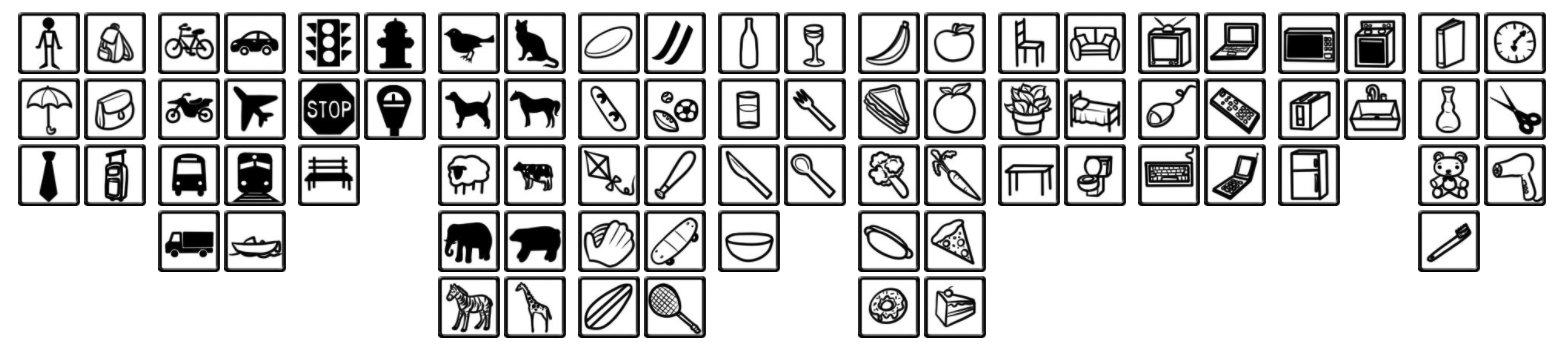
\includegraphics[width=0.9\textwidth]{img/chapters/resultados/datasets/cocodataset.png}
\caption{\label{fig:cocodataset}Categorías de objetos del dataset MS COCO}
\end{figure}

\newpage

\subsection{Open Images Dataset v4}
\label{subsec:OIDv4-dataset}

\begin{figure}[ht]
\centering
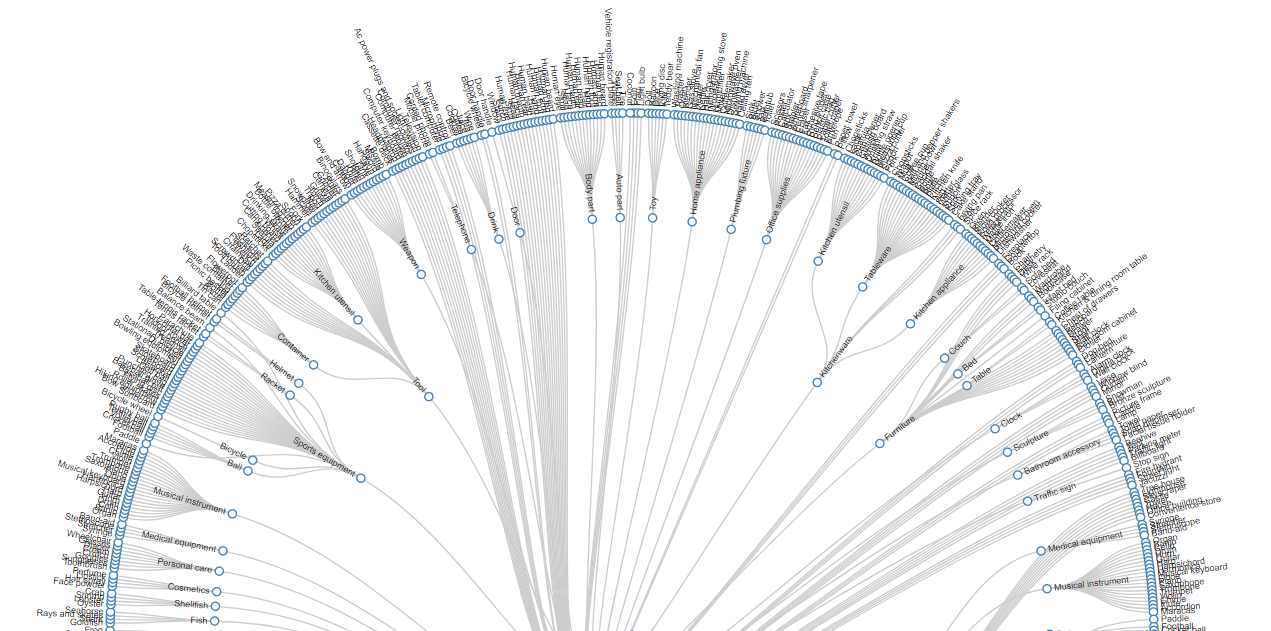
\includegraphics[width=0.7\textwidth]{img/chapters/resultados/datasets/oid-classes.png}
\caption{\label{fig:oiddataset}Categorías de objetos del dataset Open Images Dataset v4}
\end{figure}

\section{Entrenamiento YOLOv4 con Open Image Dataset v4}
\label{sec:train-openimagesv4}

\textcolor{red}{Aquí explicar como he entrenado una red neuronal con otro dataset a partir del repositorio \cite{OIDv4_ToolKit}}

\textcolor{red}{Explicar que se ha tomado 1500 imágenes de entrenamiento de las clases: person, handbag, backpack, suitcase y 300 imágenes de validación.}

\vspace{0.5cm}
\begin{lstlisting}[language=iPython,caption=Descarga dataset Open Images Dataset v4,captionpos=b,label={lst:download-oidv4}]
# Clonar el repositorio de Github
git clone https://github.com/theAIGuysCode/OIDv4_ToolKit.git
cd OIDv4_ToolKit

# Instalacion de las librerias y dependendencias
pip install -r requirements.txt

# Descarga de las imagenes de entrenamiento con un limite de 1500
python main.py downloader --classes Person Handbag Backpack Suitcase --type_csv train --limit 1500 --multiclasses 1

# Descarga de las imagenes de validacion con un limite de 300
python main.py downloader --classes Person Handbag Backpack Suitcase --type_csv validation --limit 300 --multiclasses 1

# Convertir etiquetas al formato de Darknet
python convert_annotations.py

\end{lstlisting}

\begin{figure}[ht]
\centering
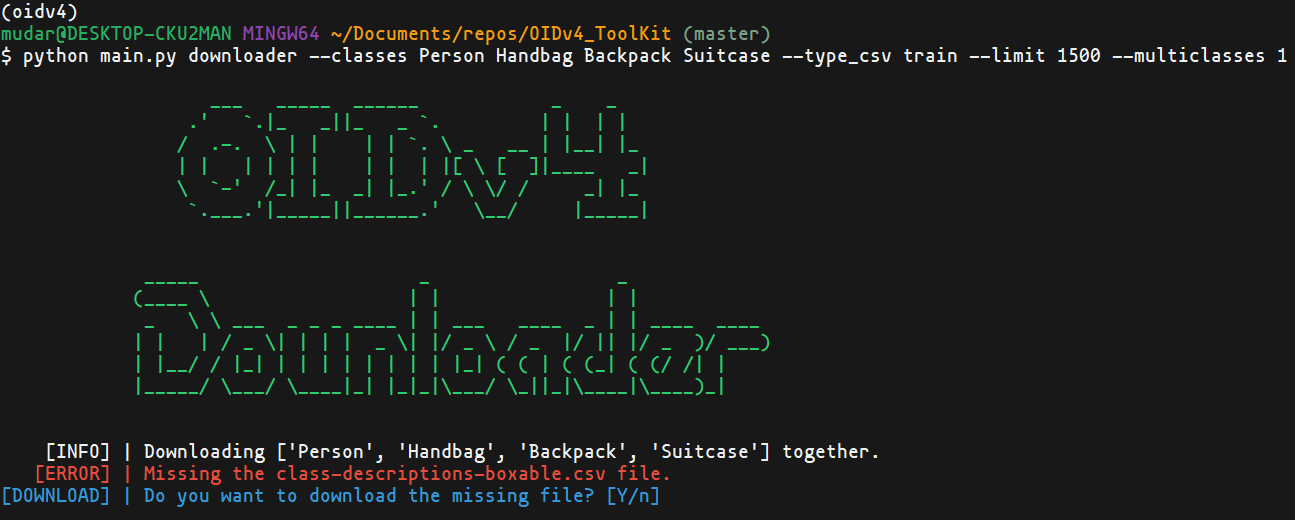
\includegraphics[width=0.55\textwidth]{img/chapters/resultados/datasets/download-oidv4.png}
\caption{\label{fig:download-oidv4}Descarga del dataset Open Images Dataset v4}
\end{figure}

\begin{figure}[ht]
\centering
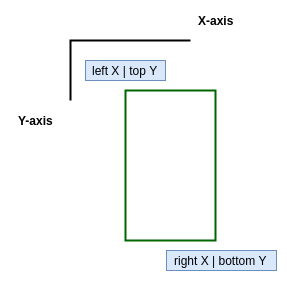
\includegraphics[width=0.45\textwidth]{img/chapters/resultados/datasets/bbox-oidv4.png}
\caption{\label{fig:bbox-oidv4}Estructura de las etiquetas de Open Images Dataset v4}
\end{figure}

La estructura que siguen las etiquetas del dataset de Open Images Dataset v4 es la siguiente:

\texttt{nombre de la clase x left top y x right bottom y}

\aviso{Aquí especificar que se utilizará MS COCO como dataset de entrenamiento de la red y se mostrará los resultados obtenidos de este entrenameinto en el capítulo de resultados}

\newpage

\section{YOLOv4 + DeepSORT}
\label{sec:desarrollo-yolov4+deepsort}

\textcolor{red}{Aquí hacer una breve descripción de deepsort, muy breve porque ya se ha explicado en el capitulo del estado del arte, y poner imagenes de su funcionamiento sobre yolov4 en el framework tensorflow}.

\newpage

\section{Algoritmo de detección de objetos abandonados}
\label{sec:algoritmo-object-detection}

\textcolor{red}{Dibujar el esquema que voy a seguir para determinar cuando un objeto ha sido abandonado.}
\url{https://app.diagrams.net/}

\textcolor{red}{Intentar meter toda la chicha posible. Que quede pendiente meter aquí código de lo que he implementado para que no quede todo en el aire y se vean de repente los resultados, por lo menos que se vea la función que hace la asociación de persona objeto y la función que establece si la persona ha abandonado un objeto o si el objeto esta abandonado y sin propietario.}

\newpage

\section{Conclusiones}
\label{sec:conclu-desarrollo}

\textcolor{red}{Hacer unas breves conclusiones de lo que se ha conseguido en base a los objetivos que se han marcado en la introducción de este capítulo \ldots}

\begin{algorithm}[H]
 \caption{How to write algorithms}
 \label{alg:howto}
 \KwData{this text}
 \KwResult{how to write algorithm with \LaTeX2e }
 initialization\;
 \While{not at end of this document}{
  read current\;
  \eIf{understand}{
   go to next section\;
   current section becomes this one\;
   }{
   go back to the beginning of current section\;
  }
 }
\end{algorithm}